\section{Design Audit: Backbones, Normalization, and Covariates}\label{app:design}

This appendix documents the component-level audit that underpins the comparison
protocol of \Cref{sec:empirical}. Three principles govern every block:

\begin{enumerate}
\item \textbf{Normalization separation.} Every backbone has its built-in
  instance normalization removed (e.g., \texttt{use\_norm=False}), and
  normalization is injected \emph{only} through the five external arms
  (\rawm{}, RevIN, SAN, FAN, CondNorm). Each backbone's ``published'' form is
  recovered by one of these arms, as \Cref{tab:audit} records. This
  component-controlled design follows the methodology advocated by benchmark
  studies \citep{qiu2024tfb}.
\item \textbf{Covariate symmetry.} Within a comparison block, all arms receive
  the \emph{identical covariate information set}; arms differ only in
  \emph{where} that information enters (backbone input versus the
  normalization restoration path).
\item \textbf{Block self-containment.} Rows from different blocks
  (\Cref{tab:blocks}) are never compared numerically in one table, because
  training budgets differ across blocks (epoch caps: Block~A 12, Block~B 15).
  All conclusions are within-block.
\end{enumerate}

\begin{table}[t]
\centering
\caption{Backbone correspondence audit. ``Published $\approx$ arm'' states
which of our external normalization arms reproduces the model as published;
``covariate path'' states how covariates enter in each block.}
\label{tab:audit}
\scriptsize
\setlength{\tabcolsep}{4pt}
\begin{tabular}{@{}p{2.5cm}p{2.5cm}p{2.4cm}p{1.9cm}p{2.9cm}@{}}
\toprule
Backbone & Published built-in normalization & Our treatment & Published $\approx$ arm & Covariate path \\
\midrule
RLinear \citep{li2023rlinear} & RevIN (the ``R'') & external arm & \texttt{revin} & none (A) / \texttt{linmix} features (B) \\
PatchTST \citep{nie2023patchtst} & RevIN, on by default & removed; external arm & \texttt{revin} & none (A) / PatchTST-Cov (B) \\
SegRNN \citep{lin2023segrnn} & instance norm (last-value subtraction) & removed; external arm & $\approx$\,\texttt{revin} (item~1) & none (A) / SegRNN-Cov (B) \\
LightGBM-DMS \citep{ke2017lightgbm} & varies by practice & window z-norm arm (RevIN-equiv.) & --- & features (B) \\
iTransformer \citep{liu2024itransformer} & \texttt{use\_norm=True} (non-affine RevIN / NST) & \texttt{use\_norm=False}; external arm & \texttt{revin} & MS: covariate variate tokens (official usage) \\
TimeXer \citep{wang2024timexer} & \texttt{use\_norm=True} & \texttt{use\_norm=False}; external arm & \texttt{revin} & MS: exogenous cross-attention (design purpose) \\
\bottomrule
\end{tabular}
\end{table}

\begin{table}[t]
\centering
\caption{Comparison-block structure. Blocks are internally uniform and never
compared to each other numerically.}
\label{tab:blocks}
\resizebox{\textwidth}{!}{%
\begin{tabular}{@{}p{2.8cm}p{4.6cm}p{4.6cm}p{4.6cm}@{}}
\toprule
Block & Backbones & Covariates & Purpose \\
\midrule
A. Main grid (pre-registered) & RLinear / PatchTST / SegRNN / LGBM & no backbone input; CondNorm restoration only & pre-registered sign validation (Gate~2) \\
B. Covariate-fair & linmix / mlpmix / PatchTSTCov / SegRNNCov / LGBM+cov & past+future features, \emph{all} arms & mechanism test under information parity \\
C. SOTA-MS & iTransformer-MS / TimeXer-MS & official covariate paths (past), all arms & normalization choice on top of SOTA covariate models \\
D. SOTA-endogenous & iTransformer / TimeXer-M & none (multivariate) & backbone-robustness extension of Block~A \\
\bottomrule
\end{tabular}}
\end{table}

\paragraph{Target-channel-only normalization is the RevIN-favorable choice}
In MS mode, the published \texttt{use\_norm} implementations window-normalize
the covariate columns together with the target. Our MS adapter instead applies
the normalization arm \emph{only to the target channel}, giving covariates a
global (train-fit) z-score. This is a deliberate, conservative concession to
the RevIN arm: window-normalizing covariates would destroy exactly the level
information they carry (e.g., the absolute magnitude of NWP wind speed), which
is the mechanism this paper criticizes; injecting it into the baseline would
artificially weaken RevIN. Under the current protocol the RevIN arm retains
full access to covariate level information through the backbone input, so any
CondNorm advantage is an advantage under RevIN-favorable conditions.
Quantifying how much the published default (window-normalizing covariates as
well) costs in practice is left to future ablation.

\paragraph{Is CondNorm's dual covariate use unfair?}
CondNorm uses covariates twice: as backbone input (Blocks B/C) and in the
restoration path. This is not an information asymmetry --- the information
\emph{set} is identical across arms within each block; only the injection
point differs. Using covariates in the restoration path is the method itself,
and the comparison ``same information, different injection point'' is
precisely the research question. In Block~C, the CondNorm arm uses lead-matched
\emph{future} forecasts in the restoration path by definition of the method,
while the backbone input information (past covariates) is identical across all
Block-C arms; TimeXer and iTransformer expose no future-covariate input path,
which is why Block~B (future features for all arms) exists as the
strict-parity counterpart.

\paragraph{Known residual asymmetries}
For transparency, we list the asymmetries that remain:
\begin{enumerate}
\item Published SegRNN subtracts the \emph{last} window value rather than the
  window mean/std of our \texttt{revin} arm; the correspondence is approximate.
\item PatchTSTCov and SegRNNCov in Block~B are our minimal covariate
  extensions; no standard recipe exists for these backbones.
\item The \texttt{gefcom\_load} temperature covariate follows the ex-post
  convention of the competition \citep{hong2016gefcom}; it is identical across
  all arms.
\item Epoch caps differ across blocks (A: 12, B: 15); this is controlled by
  the no-cross-block-comparison rule.
\end{enumerate}

\section{Reproducibility Statement}\label{app:repro}

\paragraph{Repository}
All code, frozen configurations, curation pipelines, logged results, and the
pre-registration evidence trail are provided in an anonymized repository for
review\footnote{Anonymized repository for double-blind review:
\url{https://anonymous.4open.science/r/norm-boundary} (placeholder --- the
reviewer link is provided separately to the editor at submission). The
de-anonymized public repository accompanies the camera-ready version.}; this is
the repository referred to throughout the paper. The evidence directory
includes a frozen snapshot of the MLflow tracking database, so the
pre-registration ordering documented below can be verified independently of the
authors' claims.

\paragraph{Environment}
All experiments run in a \texttt{uv}-managed environment (Python 3.12,
PyTorch 2.11 with cu128 wheels) on two NVIDIA RTX 5070~Ti GPUs (Blackwell,
\texttt{sm\_120}). The exact dependency lockfile is part of the repository.

\paragraph{Determinism}
Every run fixes its seed (seeds $0$--$4$ per configuration), enables
\texttt{torch.use\_deterministic\_algorithms(True, warn\_only=True)}, and sets
\texttt{CUBLAS\_WORKSPACE\_CONFIG=:4096:8}. Data loaders use
\texttt{drop\_last=False} throughout \citep{qiu2024tfb}, and the global
z-score is fit on the training split only.

\paragraph{Experiment tracking}
All 4{,}202 runs are logged to MLflow (SQLite backend) under a single
experiment, with run names\linebreak
\texttt{\{dataset\}\_\{norm\}\_\{backbone\}\_\{h\}\_\{seed\}}. The training
entry point logs the complete configuration as parameters and the git commit
hash as a tag on every run, so any number in this paper can be traced to the
exact code state that produced it.

\paragraph{Pre-registration}
The prediction protocol of \Cref{sec:lps} was frozen in git commit
\texttt{cab17c1} \emph{before any Block-A grid run was launched}; the commit
timestamp, together with the MLflow start times of the first grid runs,
provides the ordering evidence. The frozen artifacts are: the official LPS
specification ($w=96$, LightGBM first stage, expanding chronological
cross-validation, per-channel mean), the threshold $\tau = 0.3$, and the
predicted sign of the gap (RevIN minus CondNorm test MSE) for all eight
datasets. One archival note: a later history rewrite (removing a credentials
file from tracking) preserved all commit dates; the first grid runs carry the
pre-rewrite hash of the same pre-registration commit in their MLflow tags,
with the hash correspondence documented in the repository, so the ordering
evidence remains independently verifiable.

\paragraph{Data provenance}
\emph{jeju\_wind}: Jeju Island wind generation (2021-07 to 2023-12; 21{,}720
hourly observations) paired with \emph{archived} KMA short-term NWP forecasts
retrieved from the KMA API hub. Forecasts are lead-matched to the forecast
origin: the (D$-$2)~23h issue band covers leads 26--49\,h for $h \le 24$, and
the (D$-$3)~23h band covers leads 50--73\,h for $h \le 48$, so no forecast
used at test time would have been unavailable in operation. One archive hole
(2023-06-25 to 07-04) is handled by segment-aware windowing --- windows never
span the hole and no values are interpolated. \emph{GEFCom2014} wind, load,
and solar tracks are public \citep{hong2016gefcom}; the standard LTSF datasets
(ETTh1, ETTh2, electricity, weather) are public benchmarks. All curation code
(raw to curated Parquet, with contract assertions on monotone time index and
absence of missing values) is in the repository.

\paragraph{One-command regeneration}
\texttt{make figures} and \texttt{make tables} regenerate every figure and
table in this paper from the logged results.

\paragraph{Statistical testing implementation}
The Diebold--Mariano tests \citep{diebold1995comparing} use per-origin
$h$-step-mean squared error loss series, HAC (Bartlett/Newey--West) variance
with $h-1$ lags, and the small-sample correction of \citet{harvey1997testing};
$p$-values use a $t$ distribution with $n-1$ degrees of freedom. Because the
Bartlett estimator is positive semi-definite only for bandwidths well below
the sample size, the bandwidth is capped at $n/4$, and the variance is floored
at $10^{-12}$ before studentization. Model Confidence Sets
\citep{hansen2011mcs} use the $T_{\max}$ statistic at $\alpha = 0.10$ with the
stationary bootstrap \citep{politis1994stationary}.

\section{Extension Blocks: Information-Parity and SOTA Results}\label{app:ext}

\paragraph{Block B: information parity}
\Cref{tab:covfair} reports the covariate-fair block on the four exogenous
datasets, in which \emph{every} arm --- including \rawm{} and RevIN --- receives
the identical past and future covariate features as backbone input.
CondNorm attains the lowest mean MSE for the linmix, mlpmix, and PatchTSTCov
backbones and is within $0.01$ of the best arm for the two strongest
covariate backbones (LGBM+cov and SegRNNCov), where the number of
DM-significant cells drops accordingly (3/11 and 2/11 versus 10--11/11 for the
less flexible backbones). Averaged over (dataset, horizon) cells, the
\rawm{}$-$\cnm{} gap shrinks with backbone flexibility --- linmix $+0.127$,
mlpmix $+0.052$, LGBM+cov $-0.009$ --- consistent with a flexible backbone
learning the restoration map internally when given the covariates. Crucially,
the RevIN gap does \emph{not} shrink: RevIN+cov is worse in mean MSE than \rawm{}+cov for
every backbone, the function-class constraint predicted by
\Cref{sec:theory} via the reparameterization argument of
\citet{toner2024linear} --- instance normalization removes the level
information before the backbone can combine it with the covariates.

\begin{table}[t]
\centering
\caption{Block B (covariate-fair): mean test MSE by arm and backbone on the
four exogenous datasets (mean over dataset, horizon, and seeds; bold = best
per backbone), and the number of (dataset,\,$h$) cells (out of 11) in which
CondNorm is significantly better than RevIN by the Harvey-corrected DM test on
seed-mean losses. SAN and FAN are structurally inapplicable to LGBM+cov
(declared at pre-registration).}
\label{tab:covfair}
\begin{tabular}{@{}lrrrrrc@{}}
\toprule
Backbone & \rawm{} & RevIN & SAN & FAN & CondNorm & DM sig.\ /11 \\
\midrule
LGBM+cov     & \textbf{0.127}  & 0.146  & ---    & ---    & 0.1361 & 3 \\
linmix       & 0.2762 & 0.2967 & 0.3191 & 0.4332 & \textbf{0.1496} & 10 \\
mlpmix       & 0.1963 & 0.2201 & 0.2402 & 0.4057 & \textbf{0.1443} & 10 \\
PatchTSTCov  & 0.2851 & 0.2889 & 0.3378 & 0.3729 & \textbf{0.1434} & 11 \\
SegRNNCov    & \textbf{0.1312} & 0.1425 & 0.1822 & 0.2912 & 0.1352 & 2 \\
\bottomrule
\end{tabular}
\end{table}

\paragraph{Block C: SOTA covariate models}
\Cref{tab:sota} (top two panels) reports the SOTA-MS block, in which
TimeXer \citep{wang2024timexer} and iTransformer \citep{liu2024itransformer}
consume covariates through their official paths (exogenous cross-attention and
covariate variate tokens, respectively) with built-in normalization removed
and the five external arms injected. CondNorm is the best arm on all four
exogenous datasets for both models; the mean RevIN$-$CondNorm gap is
$+0.4122$ for TimeXer-MS and $+0.4282$ for iTransformer-MS (55 pairs each).
The applicability boundary is therefore not an artifact of weak backbones: it
persists on top of state-of-the-art covariate architectures.

\paragraph{Block D: endogenous SOTA}
The bottom panel of \Cref{tab:sota} extends Block~A's backbone set with
endogenous (multivariate, no covariate input) iTransformer and TimeXer-M runs.
The qualitative pattern of \Cref{sec:empirical} is unchanged: CondNorm wins on
the exogenous datasets and loses clearly on the standard LTSF datasets, where
instance normalization (RevIN/SAN \citealp{kim2022revin,liu2023san}, and FAN
\citealp{ye2024fan}) remains the right choice --- exactly as the LPS-based rule
predicts. Gate~2 was judged on the pre-registered Block-A backbones
only; Blocks C/D are post-registration robustness extensions.

\begin{table}[t]
\centering
\caption{Blocks C and D (SOTA extensions): mean test MSE by dataset and arm
(bold = best per row). Top: TimeXer-MS and iTransformer-MS with official
covariate paths (Block~C). Bottom: endogenous extension (Block~D), arm means
over horizons and seeds. No cross-block numeric comparison is intended.}
\label{tab:sota}
\begin{tabular}{@{}lrrrrr@{}}
\toprule
Dataset & \rawm{} & RevIN & SAN & FAN & CondNorm \\
\midrule
\multicolumn{6}{@{}l}{\emph{Block C: TimeXer-MS (gap $+0.4122$, 55 pairs)}} \\
gefcom\_load  & 0.355  & 0.3249 & 0.3238 & 0.3434 & \textbf{0.104}  \\
gefcom\_solar & 0.1784 & 0.1778 & 0.2491 & 0.191  & \textbf{0.057}  \\
gefcom\_wind  & 1.027  & 1.0772 & 1.0502 & 1.0513 & \textbf{0.1668} \\
jeju\_wind    & 0.6561 & 0.688  & 0.6529 & 0.6864 & \textbf{0.2989} \\
\midrule
\multicolumn{6}{@{}l}{\emph{Block C: iTransformer-MS (gap $+0.4282$, 55 pairs)}} \\
gefcom\_load  & 0.3606 & 0.3288 & 0.3122 & 0.347  & \textbf{0.1053} \\
gefcom\_solar & 0.1901 & 0.1784 & 0.229  & 0.1865 & \textbf{0.0567} \\
gefcom\_wind  & 1.0267 & 1.1226 & 1.0449 & 1.0604 & \textbf{0.1658} \\
jeju\_wind    & 0.6775 & 0.7036 & 0.664  & 0.6942 & \textbf{0.3012} \\
\midrule
\multicolumn{6}{@{}l}{\emph{Block D: iTransformer (endogenous)}} \\
electricity   & 0.1341 & 0.1314 & \textbf{0.13}   & 0.1339 & 0.2096 \\
etth1         & 0.4413 & \textbf{0.3826} & 0.3857 & 0.3976 & 1.4851 \\
etth2         & 0.6742 & 0.3037 & \textbf{0.3002} & 0.3329 & 3.4686 \\
gefcom\_load  & 0.3524 & 0.3364 & 0.3251 & 0.3524 & \textbf{0.1074} \\
gefcom\_solar & 0.1808 & 0.1774 & 0.1778 & 0.1837 & \textbf{0.0569} \\
gefcom\_wind  & 1.0399 & 0.9734 & 0.9781 & 1.0844 & \textbf{0.1586} \\
jeju\_wind    & 0.6963 & 0.7242 & 0.694  & 0.6984 & \textbf{0.2974} \\
weather       & 0.1907 & 0.1706 & \textbf{0.168}  & 0.17   & 0.6992 \\
\midrule
\multicolumn{6}{@{}l}{\emph{Block D: TimeXer-M (endogenous)}} \\
etth1         & 0.3962 & \textbf{0.3805} & 0.3895 & 0.4309 & 1.4821 \\
etth2         & 0.4838 & 0.2946 & \textbf{0.2897} & 0.3815 & 3.5344 \\
\bottomrule
\end{tabular}
\end{table}

\paragraph{Qualitative behavior}
\Cref{fig:samples} illustrates the mechanism behind the aggregate numbers on
held-out test windows. During wind ramps, RevIN anchors the forecast to the
lookback-window statistics and systematically lags or misses the ramp, whereas
CondNorm restores the level from the lead-matched NWP forecast and tracks it.
On overcast solar days, RevIN restores the level of the (sunny) input window,
while CondNorm's covariate-conditional restoration adjusts the level downward
to the forecast irradiance regime. The standard-benchmark rows (etth1, etth2,
weather) show CondNorm's failure mode outside the applicability boundary: its
covariate-conditional restoration places the forecast at a visibly wrong
level.

\begin{figure}[t]
\centering
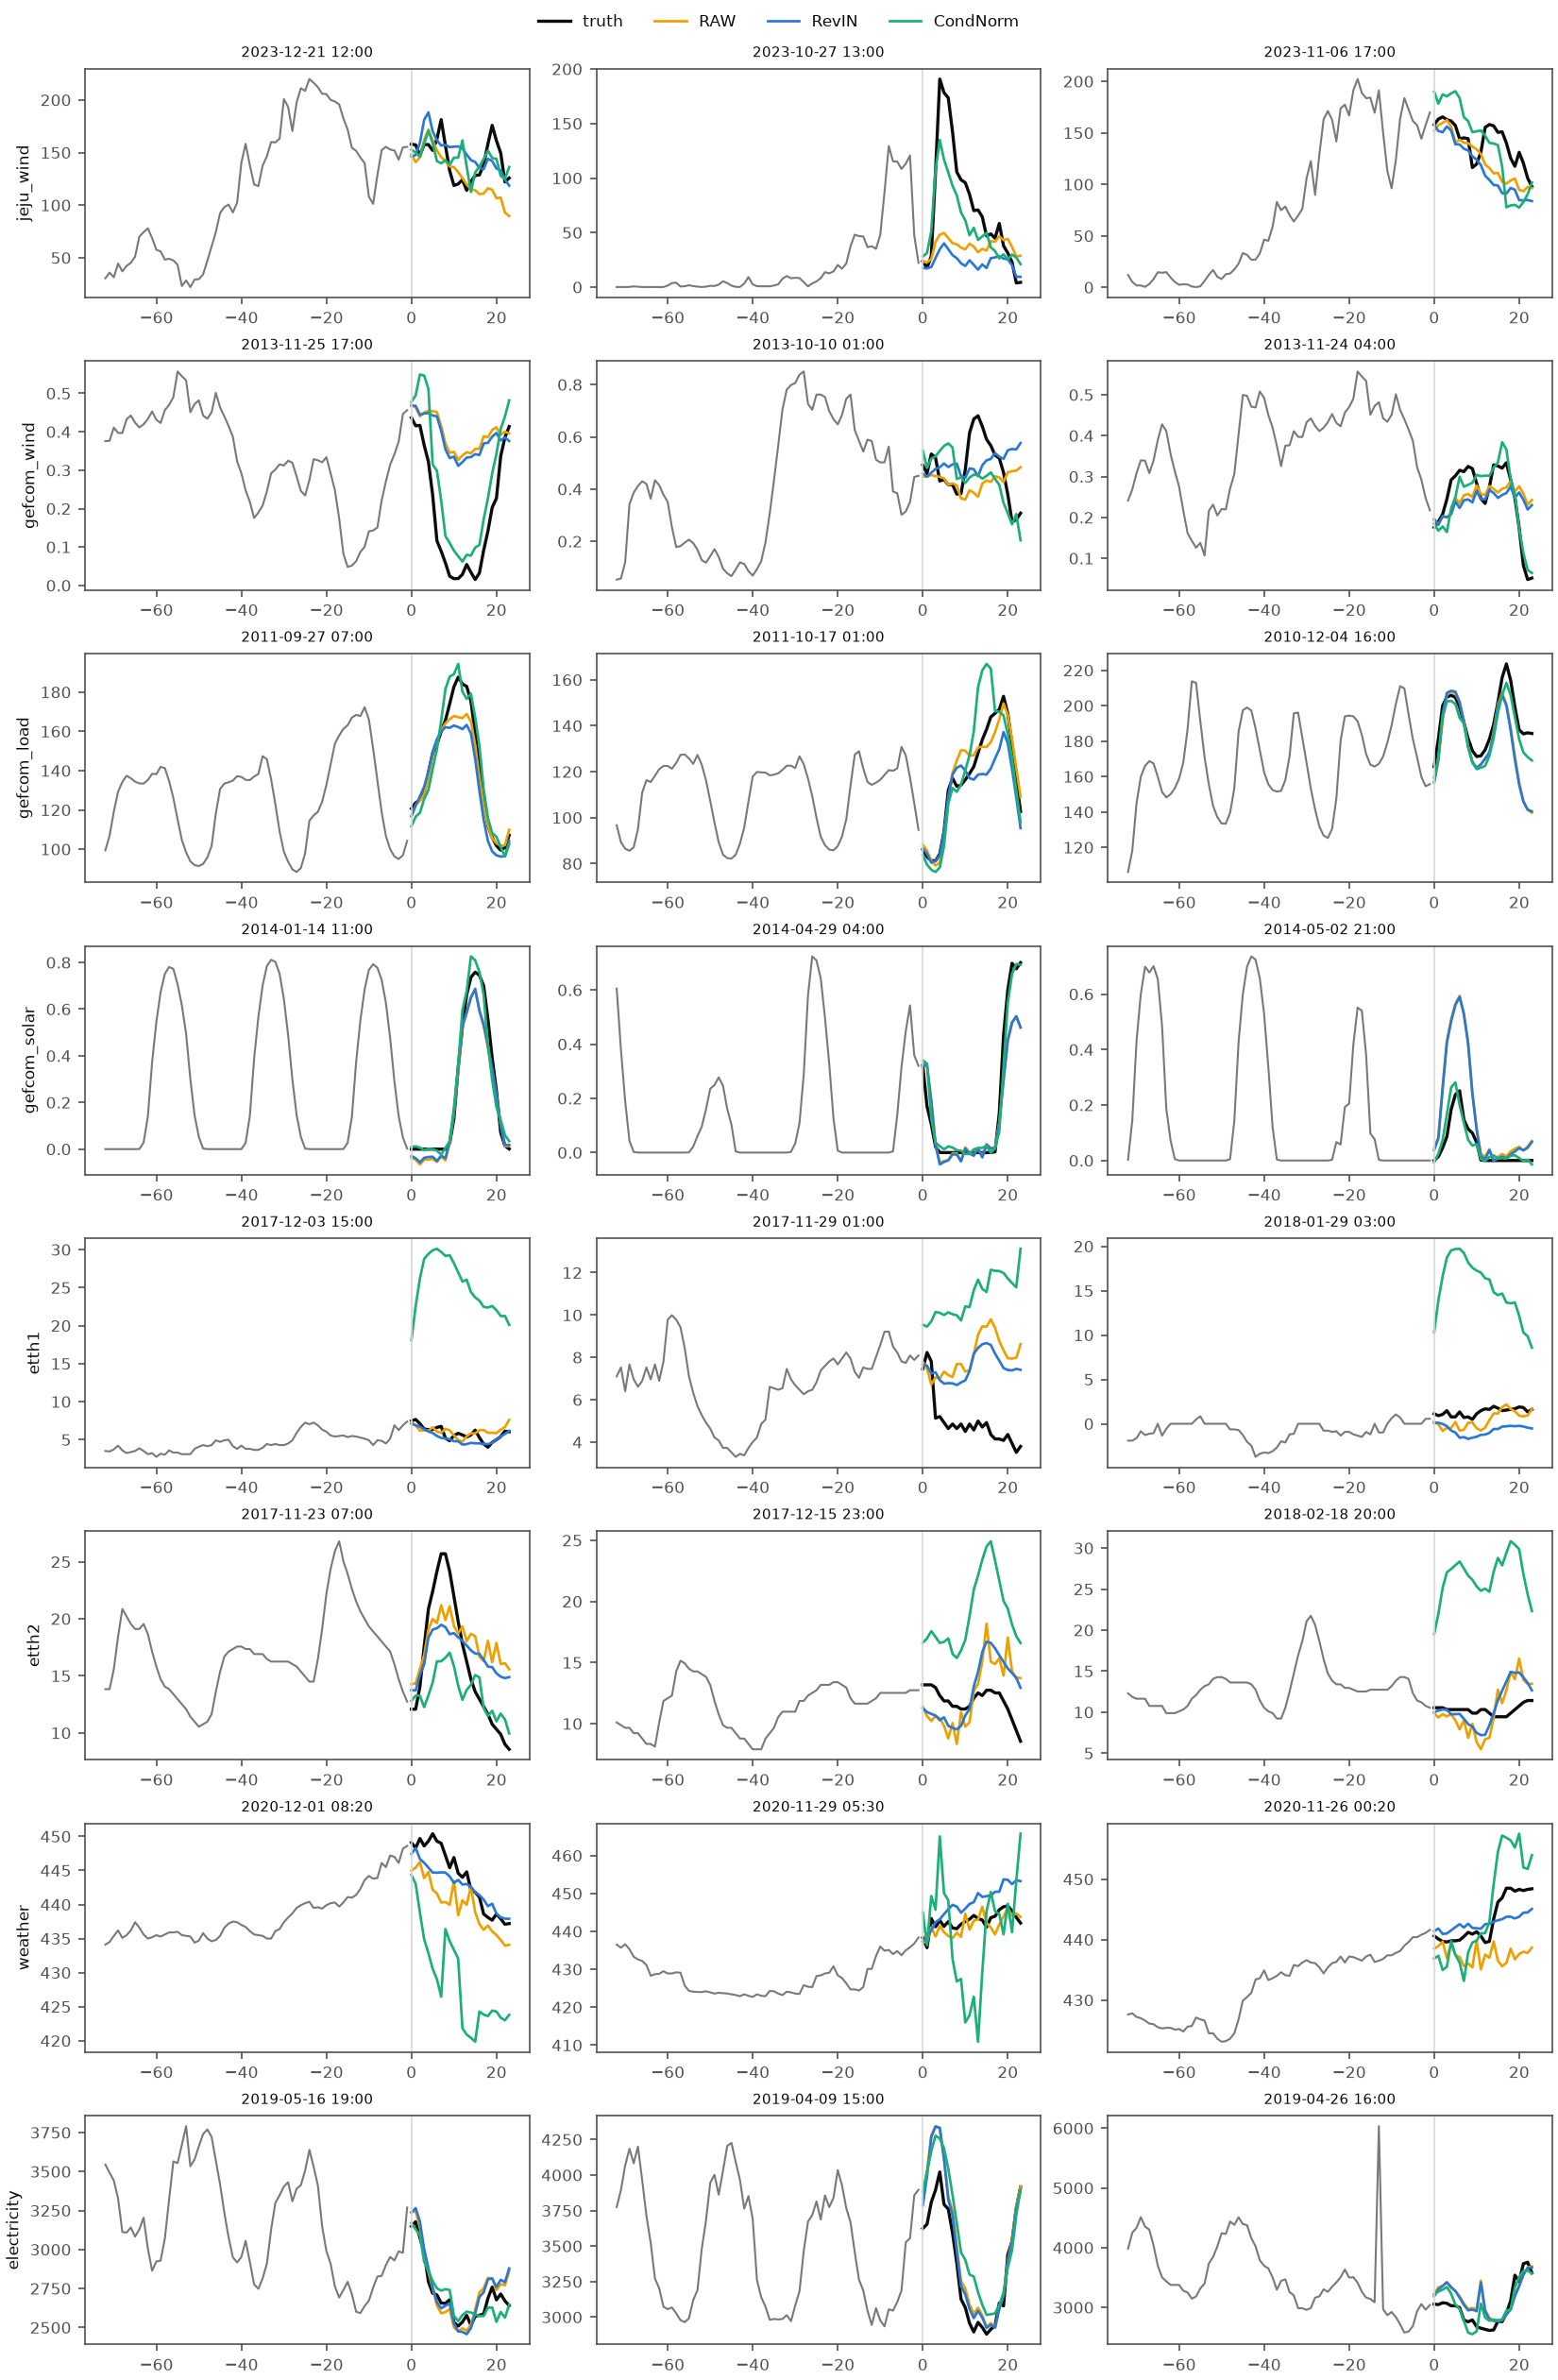
\includegraphics[keepaspectratio,width=\textwidth,height=0.8\textheight]{figures/sample_forecasts.png}
\caption{Qualitative test-set examples (identical backbone and information
set): one row per dataset, three sample windows per row; grey is the lookback,
black the ground truth, and colored lines the \rawm{}, RevIN, and CondNorm
forecasts. See the accompanying text for the reading of the wind, solar, and
standard-benchmark rows.}
\label{fig:samples}
\end{figure}
